\documentclass[12pt]{article}
\usepackage[T2A]{fontenc}			% кодировка
\usepackage[utf8]{inputenc}			% кодировка исходного текста
\usepackage[english]{babel}	
\usepackage{tikz}
\usepackage{fontspec}
\setmainfont{Times New Roman}
\linespread{1.3}

\usepackage{bookmark}
\usepackage{lscape}
\usepackage{lmodern}
\usepackage{amssymb,amsmath}
\DeclareMathOperator{\EX}{\mathbb{E}}% expected value
\usepackage{geometry}
\geometry{
	a4paper,
	left=20mm,
	top=20mm,
	right = 20mm, 
	bottom = 20mm
}
\usepackage{graphicx,grffile}
\usepackage{floatrow}
\floatsetup[table]{capposition=top}

\usepackage{pgfplots}
\usepackage{pgfplotstable}
\usepackage{graphicx}
\usepackage{indentfirst}
\usepackage[backend=biber, bibencoding=utf8, sorting=nty, maxcitenames=2, bibstyle=apa, style=authoryear]{biblatex}
\addbibresource{bibliography.bib}
\renewcommand*{\nameyeardelim}{\addcomma\space}

\usepackage{hyperref}
%\usepackage[usenames,dvipsnames,svgnames,table,rgb]{xcolor}
\hypersetup{
	colorlinks=true,       	% false: ссылки в рамках; true: цветные ссылки
	linkcolor=magenta,          % внутренние ссылки
	citecolor=blue,        % на библиографию
	filecolor=magenta,      % на файлы
	urlcolor=magenta          % на URL
}


\begin{document}
	
	\begin{titlepage} % Suppresses displaying the page number on the title page and the subsequent page counts as page 1
		\newcommand{\HRule}{\rule{\linewidth}{0.5mm}} % Defines a new command for horizontal lines, change thickness here
		
		\begin{center}
			

		
		
		%------------------------------------------------
		%	Logo
		%------------------------------------------------
		
		
		
\includegraphics[width=0.8\textwidth]{logo_hse.eps}\\[4cm] % Include a department/university logo - this will require the graphicx package
		
		%----------------------------------------------------------------------------------------
		
		%------------------------------------------------
		%	Headings
		%------------------------------------------------
		
		%\textsc{\Large National Research University}\\[0.5cm] 
		
		
		%------------------------------------------------
		%	Title
		%------------------------------------------------
		
		{\large \bfseries Final project}\\[1cm]

		
		{\LARGE  Risk preferences and cheating behavior}\\[0.5cm]
		

		


		
		%------------------------------------------------
		%	Author(s)
		%------------------------------------------------
		
	
			\textit{Author:}\\
			Maksim \textsc{Peshkov} \\[2cm]

			% Your name
	
		
		
		\textbf{Abstract}

		\end{center}

	This paper examined the impact of risk preferences on dishonesty. To estimate risk aversion, it was used two methods: self-reported perception of risk and the Holt-Laury procedure. The design of "mind game" was the foundation to measure deception level. In the experiment it was played the lottery before each round of "mind game" to estimate the short-term effect of last experience with taking risk to its perception, according to which there were introduced three self-selected groups: incentivized, discouraged and control. Treatments of experiment are based on the randomly chosen pair of numbers in each round (pairs vary in difference between numbers). Experiment design provides the analysis of risk seeking as incentive to dishonesty and examine simultaneous influence on deception level by last experience in game with taking risk and the outcome difference. Results show that risk seekers are cheat more, though the measurement by Holt-Laury procedure is not significant, which could be caused by sample characteristics. Furthermore, it was found the impact of last experience on perception of risk and decision to behave unethically, in which for treatments with the lowest payoff for honest behavior deception level in incentivized group is the highest and in discouraged group it is the least. Finally, outcome difference in treatments has negative influence on the impact from last experience with taking risk, so higher difference leads to decrease the deterrent effect in discouraged group and more cheating level.

		
	
		\vfill % Push the date up 1/4 of the remaining page
		
	\end{titlepage}

	\section{Introduction}
	\vspace{-0.4cm}
	
	The topic of dishonest behavior has been widely discussed in the academic literature. There are many reasons for deception, such as attention to moral standards \autocite{mazar2008dishonesty}, and the importance of a reputation as an honest person \autocite{ayal2015three, abeler2019preferences}. One of the first works on this topic demonstrated in a theoretical model that risk preference is an important factor for cheating \autocite{becker1968crime}. \cite{arneklev1993low, zimerman2014self} confirmed it empirically and showed that risk-taking measured by self-reported questionnaires is one of the most essential components of unethical behavior. However, dishonest behavior and risk preferences are difficult to measure. Therefore, there are different methods for more accurate calculation. The concept of "mind game" is used for the level of cheating, which can reduce the bias of self-reported deception assessment and roughly estimate the average level of dishonesty, although this method cannot show the exact number of cases of dishonest behavior \autocite{jiang2013cheating, mol2020not}. On the other side, measuring perception of risk is also difficult because people can behave differently in some situations. To solve this problem, 	\cite{holt2002risk} offered the task with 10 rounds of binary choice (more risky and less risky). This measurement is more accurate and used in many papers  (see, for example, \cite{jamison2008deceive, rigby2015contract,bejanyan2021financial}). 
	
	Furthermore, the choice to behave unethically is influenced by some factors. \cite{gneezy2005deception, gneezy2018lying} demonstrated that people are sensitive to their gains when deciding to lie. When the lying costs are higher and payoff is lower, participants did not want to cheat, whereas if participants saw that they could take risks and make more money, they might be more confident and incentivized to take risks or engage in dishonest behavior. Furthermore,  \cite{zimerman2014self} found difference in deception level of incentivized persons and discouraged, which is explained by positive correlation between risk-seeking and dishonest behavior. In their experiment there were 2 treatments and participants knew their groups before estimation of cheating behavior, though deceptive choice is also effected by last reward and risk preferences could be changeable. Consequently, it is necessary to examine the effect of consequences of the last game to ethical choice, which could be different to incentivized and discouraged treatments varied by the amount of reward.
	
	The purpose of this paper is to expand existing literature about cheating behavior by analyzing the impact of risk perception on the level of dishonesty, using the concept of "mind game" to estimate deception and the Holt-Laury task to measure risk aversion. On the other side, this work will extend the results of previous papers about the significance of consequences for cheaters to unethical behavior by analyzing three treatments (incentivized, discouraged and control), which are varying by rounds and the amount of possible reward for each participant. Furthermore, it would be analyzed the simultaneous impact of outcome difference and last payoff in the lottery on lying costs and unethical behavior. The rest of this paper organized as follows. The next section presents literature review. The section \ref{design} introduces experimental design and hypotheses. Last section \ref{results} shows preliminary results.
	
	
	\section{Literature review}\label{lit}
	
	 Deviant behavior is an important object of research for psychologists and economists. One of the first article discussing the reasons and instruments to negotiate unethical behavior was \cite{becker1968crime}. In this paper author examined the enforcement to deter the level of criminal behavior. He deployed the general model of illegal activities and claimed that offenders are "risk preferers", so to neglect criminal behavior it is optimal to make crime "would not pay" when the possible outcomes of illegal activities are less than in legal ones. This model was the foundation of \textit{A General Theory of Crime} by \cite{gottfredson1990general}. Authors investigated the determinants of imprudent behavior focusing on individual differences in self-control. \cite{arneklev1993low} explored the link between low self-control and unethical behavior. Authors found that risk-seeking is one of the most important factor to behave imprudently. However, they used self-reported perception of risk, which would be inaccurate, because people usually overestimated their risk preferences, though most of them are risk averse \cite{kai1979prospect}. To decrease this bias, \cite{holt2002risk} demonstrated the innovative method to estimate it in 10 rounds with a set of paired lottery choices. Using this task, authors found that participants are frequently risk averse and claimed that questionnaire responses and decisions in hypothetical and low monetary reward environments did not well predict decisions in higher monetary payoff environments. Therefore, it is necessary that the lottery questionnaire to measure risk aversion and the decision-making questionnaire to estimate dishonesty, for example, have nearly identical rewards.
	 
	 Measuring dishonest behavior has been discussed by many scientists, because moral standards or beliefs could affect to choose dishonest behavior. \cite{tversky1974judgment} considered that humans make predictable errors of judgement when forced to deal with ambiguous evidence or make challenging decisions, for example, decisions connected with their reputation as honest persons. Consequently, the investigation of dishonest behavior by survey methods led to underestimated cheating rate because people faced with challenging decision to show themselves as dishonest, which can lead to reputation costs.
	 To solve this problem, there was considered the assessment without self-reported information.  \cite{kerkvliet1994cheating} used the randomized response (RR) questionnaire in hopes of eliciting more truthful responses from students when queried about cheating. The main idea was to estimate the cheat level as deviation from the distribution when all students are honest. He found that this method is more applicable to estimate cheat level when direct questionnaire (DQ). Moreover, it laid the foundation to use \textit{foresight} in further articles.
	 For instance,  \cite{jiang2013cheating} designed the first "mind game", when the participants should choose the side of  dice (Up or Down) and could change the choice after or before roll. Due to estimation of binary \textit{foresight} (1 when participant said the highest number) authors compared the cheating level in two variants of mind games. They found more deception when participants made choice after rolling, and this variant is more appropriate to estimate cheating rate and analyze its reasons. This article showed new exploration in mind games and their importance to assess dishonesty, though it did not clearly explain the questions about stimulus.
	 \cite{abeler2019preferences} explored main papers about incentives to dishonest behavior and repeated their results, including "mind games". They emphasized that a preference for being seen as honest and a preference for being honest are the main motivations for truth telling, which is approved in empirical and theoretical framework. However, they did not explore the effect of risk preferences measuring by Holt-Laury task, which should give more accurate assessments.
	 
	 Other problem to evaluate the dishonest behavior and the importance of risk seeking is the significance of last results in game with taking risk, when the loss could play the role of sanction and decrease the incentives to dishonest behavior. One of the first paper examined this issue was \cite{tittle1973moral}, in which it was investigated the impact of sanctions on cheating level and compared it with moral standards among students. They approved the deterrence theory, when the threat of punishment will deter people from committing crime. In fact, not only the threat of punishment has an impact, but also the opportunity benefits and costs. \cite{gneezy2005deception} demonstrated that in dictator game participants cheated less than they would win less. Other verification was in \cite{zimerman2014self} using the concept of "mind game". They found more deception level among incentivized participants, who could win more money for cheating. In addition, the results of this article showed positive correlation between self-reported perception of risk and deception level, which is more in incentivized treatment. The effects of possible outcomes and risk preferences were analyzed in \cite{gneezy2018lying}. They emphasized three different ways to measure the size of lying costs (three main factors to behave dishonestly): "the payoff dimension (monetary gains of lying), the outcome dimension (the distance between what the agent observes and what he says), and the likelihood dimension (the ex ante probability that the agent’s report is true)" \autocite{gneezy2018lying}. In other papers these effects were observed too. The influence of possible payoffs and risk preferences was partially analyzed in \cite{mol2020not}. Authors examined the effects of "being observed" and "being watched" in Virtual Reality. They concluded that when participants are observed, they cheat less in "mind game", because the risk and lying costs are higher. However, all of these papers did not examine the significance of last result in game with taking risk on unethical decisions, when participants could be incentivized or discouraged in each round and change their risk preferences in different scale depending on the possible reward/loss in the last experience.
	 
	 This paper aims to examine the importance of risk preferences to dishonest behavior. The foundation of the experiment is "mind game"  similar to the game in  \cite{mol2020not}. To measure risk preferences, I use Holt-Laury task set by \cite{holt2002risk} and self-reported risk preferences in the questionnaire. The analysis of effect by different perceptions of risk in 3 groups on cheat level is based on the created lottery with two options in each round (safe and risky), which is described below. This design should expand the literature about the importance of consequences for cheaters in \cite{gneezy2005deception, zimerman2014self, gneezy2018lying}, because in each round participant could be in any group and his or her risk preferences depends on consequences of previous outcome in the lottery in each round, which also have influence on deceptive choice. Moreover, in this work I try to analyze simultaneous effects by outcome difference and payoff in last game (lottery), which would open new discussion about simultaneous impacts on lying costs.

	\section{Experimental design}\label{design}
	
	The experiment was run on online platform (\href{https://cheatriskgame.herokuapp.com/join/pububagu}{Link to my experiment in Heroku}) and divided into 3 blocks: survey, the Holt-Laury task and lottery with "mind game" repeated  in 8 rounds.
	In the first page participants should write personal ID if they are students of Behavioral and Experimental Economics (Fall 2021) course. Otherwise, they could write any random number more than 1000. Before the beginning of each block, there was the instruction in which it was described what they would do further. In each round they could win some money, which was explained in instructions. In the final page they won the number from the random chosen round. 
	
	Each block has own goal and provides collecting data to test different hypotheses, which is described below. It is necessary to emphasize that in my research treatments are not stable for all rounds. In each round all participants were randomly divided into 3 treatments with different numbers in the final block: (2, 6), (6, 12), (2, 12). Also, there was self-selected division into 3 groups based on the decision and result of the lottery with binary choice in each round: picking safe option, selecting risky option and won the least number (lost), selecting risky option and won the highest number.
	
	\subsection{Survey}
	In the first part I collected personal information about participants. The following questions with possible answers were asked.

	\begin{itemize}\vspace{-0.2cm}
		\item What is your age?
		
		Participants should write their age and in this question there was not any variants to choose. In the analysis this variable is called as  \textit{age}.
		\vspace{-0.2cm}
		\item What is your gender? 
		
		There were two possible answers: Male or Female. Participants should choose one of them. In the analysis this variable is called as  \textit{sex}, where 'Male' is equal to 1, 'Female' is equal to 0.
		\vspace{-0.2cm}
		\item What is your monthly income?
		
		There were six possible answers:
		\vspace{-0.3cm}
			\begin{enumerate}
				\item <10 000 rubles \vspace{-0.2cm}
				\item 10 000 - 20 000 rubles \vspace{-0.2cm}
				\item 20 000 - 40 000 rubles \vspace{-0.2cm}
				\item 40 000 - 70 000 rubles \vspace{-0.2cm}
				\item 70 000 - 100 000 rubles \vspace{-0.2cm}
				\item >100 000 rubles \vspace{-0.2cm}
			\end{enumerate}
	
	Participants should choose one of them. In the analysis this variable is called as \textit{income} and the category is range from 1 to 6 as it follows above.
	
	\item What is your cumulative GPA (rounded)?
	
	In the screen participants could see 10 numbers from 1 to 10. They should choose one of them. In the analysis this variable is called as \textit{gpa} and the category is range from 1 to 10.
	
	\item How often do you cheat at university? (10 - always, 1 - never)
	
	In the screen participants could see 10 numbers from 1 to 10. They should choose one of them. In the analysis this variable is called as \textit{cheat activity} and the category is range from 1 to 10.
	
	\item Do you agree that cheating behavior is wrong? (10 - absolutely agree, 1 - absolutely disagree)
	
	In the screen participants could see 10 numbers from 1 to 10. They should choose one of them. In the analysis this variable is called as  \textit{cheat disagreement} and the category is range from 1 to 10.
	
	\item How do you see yourself: Are you generally a person who is fully prepared to take risks or do you try to avoid taking risks? (1 - risk averse, 10 - fully prepared to take risks)
	
	In the screen participants could see 10 numbers from 1 to 10. They should choose one of them. In the analysis this variable is called as  \textit{subject risk} and the category is range from 1 to 10.
		
	\end{itemize}
	
	Self-reported risk preferences (variable \textit{subject risk}) is one of the most important variable. \cite{arneklev1993low, zimerman2014self} found more deception among risk-seekers, where the data was collected by questionnaires. Therefore, in this paper I assume to find the same results for cheat level measuring by average  \textit{foresight} in "mind games".
	
	\vspace{0.2cm}
	
	\textbf{Hypothesis 1:}
	\textit{Self-reported risk seeking has positive influence on deception level in "mind games".}
	
	Moreover, collected data includes information about students' cheat activity and disagreement. There are some papers, in which authors used self-reported level of unethical behavior \autocite{tittle1973moral, kerkvliet1994cheating}. Although I found this estimation inaccurate, but also I assume it would be found the same results for the dependent variable \textit{cheat activity} as for the measuring dishonesty in "mind games". This hypothesis is based on the \cite{kerkvliet1994cheating}, in which authors examined not significant difference between DQ and RR.
	
	\vspace{0.2cm}
	
	\textbf{Hypothesis 2:}
	 \textit{The results in regressions when the dependent variable is self-reported cheat activity and when the response variable is the foresight in "mind games" do not differ significantly.}
	
	Information about age, sex, income and gpa are individual characteristics which I use in regressions as control variables. However, in literature there is discussion about their influence on dishonesty. In most papers there were demonstrated that deception level higher for younger, poorer, less educated males \cite{mol2020not, zimerman2014self, kerkvliet1994cheating, arneklev1993low}. In this paper I test the same hypotheses.
	
	\vspace{0.2cm}
	
	\textbf{Hypothesis 3a:}
	\textit{Age has negative influence on deception level in "mind games".}
	
		\textbf{Hypothesis 3b:}
	\textit{Income has negative influence on deception level in "mind games".}
	
		\textbf{Hypothesis 3c:}
	\textit{GPA has negative influence on deception level in "mind games".}
	
		\textbf{Hypothesis 3d:}
	\textit{Deception level in "mind games" is higher among males.}
	\vspace{-0.2cm}
	
	\subsection{Holt-Laury task}

	After survey participants should complete the Holt-Laury task set by \cite{holt2002risk}, after which they did not win anything. In the task there are 10 questions with paired lottery choices. These pairs are structured so that the lesser payoff in choice “A” is always worth more than the lesser payoff in choice “B”. Initially, the chance of the high payoff is 1/10 and the low payoff 9/10. With each step, the probability of the high payoff steadily increases by 1/10. When the probability of the high payoff is low, choosing the “B” lottery is seen as the risky decision. As the probabilities change, the expected value of “B” over “A” increases. When this occurs, continuing to choose the “A” lottery indicates risk aversion. 

	Before the beginning of the Holt-Laury task participants got this instruction with the example of binary choices: 
	
	\textit{To begin with, you will complete the Holt-Laury task to provide information about your risk preferences. In 10 questions you should choose one of two options. Each option demonstrates two numbers with probabilities of falling.
		For instance, you can choose between (20\% chance of \$15 or 80\% chance of \$10) and (20\% chance of \$30 or 80\% chance of \$1). It means that in the first variant \$15 will fall with a 20\% probability and \$10 will fall with an 80\% probability, whereas in the second variant \$30 will fall with a 20\% probability and \$1 will fall with an 80\% probability. Which one do you prefer more? This is the main question that you must answer 10 times with different options.}


\begin{table}[!ht]
	\caption{Options A and B in the Holt-Laury task and categories of risk preferences}
	\label{optionsholt}
	\centering
	\footnotesize
	\begin{tabular}{|c|c|c|c|}
		\hline
		Option A &  Option B & $\EX$(A)-$\EX$(B) & Category of risk preferences\\ 
		&&&(option B in the first time)\\
		\hline
		10\% chance \$20 or 90\% chance \$16 & 10\% chance \$38 or 90\% chance \$1 & 9.9 &10\\ 
		20\% chance \$20 or 80\% chance \$16 & 20\% chance \$38 or 80\% chance \$1 & 8.4 &9\\ 
		30\% chance \$20 or 70\% chance \$16 & 30\% chance \$38 or 70\% chance \$1 & 5.1 &8\\ 
		40\% chance \$20 or 60\% chance \$16 & 40\% chance \$38 or 60\% chance \$1 &1.8 &7\\ 
		50\% chance \$20 or 50\% chance \$16 & 50\% chance \$38 or 50\% chance \$1& -1.5 &6\\ 
		60\% chance \$20 or 40\% chance \$16 & 60\% chance \$38 or 40\% chance \$1&-4.8 &5\\ 
		70\% chance \$20 or 30\% chance \$16 & 70\% chance \$38 or 30\% chance \$1& -8.1 &4\\ 
		80\% chance \$20 or 20\% chance \$16 & 80\% chance \$38 or 20\% chance \$1& -11.4 &3\\ 
		90\% chance \$20 or 10\% chance \$16 & 90\% chance \$38 or 10\% chance \$1 &-14.7 &2\\ 
		100\% chance \$20 or 0\% chance \$16 & 100\% chance \$38 or 0\% chance \$1 &-18 &1\\ 
		\hline
	\end{tabular}
\end{table}
		
	In the Table \ref{optionsholt} there are possibilities in my Holt-Laury procedure. The categories of risk aversion were set by the first appearance of option B. Based on the difference between expected values in option A and option B the categories of 10, 9, 8 - risk seeking preferences; 7, 6 - risk neutral attitudes; 5, 4, 3, 2, 1 - risk averse preferences (the same categories was in \cite{gruener2018eliciting}). In the regression analysis this variable is named \textit{holt risk}.
	
	One of the most important factor of dishonest behavior is perception of risk, because the risk of being caught satisfies risk seekers or frightens risk averse people \autocite{arneklev1993low, becker1968crime}. However, there is a discussion how to measure risk preferences. Different assessments highly diverge, so it is necessary to use some of them to analyze the significance of risk aversion to dishonesty \autocite{gruener2018eliciting}. In the survey it was collected the data about self-reported preferences, while in this block it was collected the data by Holt-Laury procedure. Consequently, I assume to find positive correlation between the measurement of risk seeking by Holt-Laury task and the level of cheating.
	
	\vspace{0.1cm}
	
	\textbf{Hypothesis 4:}
	\textit{The estimation of risk seeking by Holt-Laury procedure has positive influence on deception level in "mind games".}
	
	\vspace{-0.4cm}
	
	\subsection{Mind game and lottery}
	\vspace{-0.1cm}
	
	This block is consist of 8 rounds with repeated procedure: 1) choose one of two options in the "lottery", 2) play the "mind game". Before each round there was randomly selected one of the pairs (a, b, a > b): (6, 2), (12, 6), (12, 2) (later in the regression analysis I coded them as 1, 2, 3 and called this variable as \textit{treatment number}). Then in the lottery players could win a,b or $\frac{a+b}{2}$ if the chosen pair was (a, b). In the "mind game" players could win a or b. In each round participant gained the sum of winning numbers in the lottery and "mind game". Before the beginning of this block, they got this instruction: 
	
	\textit{
		In the experiment you will play 8 rounds, in each of them you will play two games (each of them you can win 2, 6 or 12).}
	
	\textit{In the first game there will be two options to choose. In the first, there is a number with probability of falling (equal to 1). In the second, two possible numbers with probabilities of falling (like it was in Holt-Laury task). You would win the number which falls in your chosen variant.}
	
	\textit{In the second game you will play a "mind game". In the first stage you should choose the side "Left" or "Right" and REMEMBER it. In the second stage, you will know the left and right numbers (corresponding their sides) and should choose the number from your chosen side in the first stage. In this game you would win the number from CHOSEN side.}
	
	\textit{In the final page of round you will know your prize in this round (equals to sum of winning number). After all rounds, you will win the prize in the random chosen round.}
	
	\vspace{-0.2cm}
		
	\subsubsection{The lottery}
	
	\vspace{-0.2cm}
	
	The purpose of the lottery is to divide players into 3 groups: incentivized, discouraged and control. Division is based on the choice in the lottery with 2 options (Left or Right) (see in the Table \ref{lotteryoptions}), where (a and b) is a randomly chosen pair and a > b. 
	
	\begin{table}[!ht]
		\caption{Options in the lottery and their expected values}
		\label{lotteryoptions}
		\centering
		\footnotesize
		\begin{tabular}{|c|c|c|c|}
			\hline
			Option Left &  Option Right &$\EX$ Left&$\EX$ Right\\
			\hline
			$\$ \frac{a+b}{2} \text{ with probability } 1$ 
			& $ \begin{cases}
					\$a \text{ with probability } 0.33 \\ 
					\$b \text{ with probability } 0.67 
				\end{cases} $&$ \frac{a+b}{2}$&$ \frac{a+2b}{3}$\\
			\hline
		\end{tabular}
	\end{table}
	
	Option Left is safe option and expected value is equal to $ \frac{a+b}{2}$, while option Right is risky option and expected value is equal to $ \frac{a+2b}{3}$, which is less than in safe option, but players could win a>$ \frac{a+b}{2}$ with probability 0.33 (the prize was generated randomly with described probabilities). Therefore, in the group "choosing safe option" (control) there are players who chose option Left in the round; in the group "choosing risky option and won" (incentivized) there are players who chose option Right in the round and won a; n the group "choosing risky option and lost" (discouraged) there are players who chose option Right in the round and won b. In the regression analysis \textit{group number} variable described the player's group of each round: 1 - "choosing safe option" , 2 - "choosing risky option and won", 3 -"choosing risky option and lost". For each participant it was estimated average \textit{group number} and called \textit{average category person}.
	
	The decision to run the lottery in each round is caused by concern that risk preferences is changeable, because in different conditions lying costs are not similar for the players. Basically, \cite{zimerman2014self} demonstrated that incentivized group cheat more. However, in their experiment stimulus to earn more money from cheating was constructed before the experiment to analyze the long-term effect. In my experiment there is an analysis of short-term effect to lying costs. Moreover, the mechanism is directed to change perception of risk influencing on lying costs. When a participant won in risky option in the lottery, he or she could feel more confident and become more risk seeking, which leads to decrease lying costs and increase the probability to dishonest behavior. Otherwise, when participant lost, he or she could feel more aware and become more risk averse, which led to decrease the probability to dishonest behavior. Therefore, I assume the difference in deception level between groups and test these hypotheses.

	
	\vspace{0.2cm}
	
	\textbf{Hypothesis 5a:}
	\textit{In incentivized group deception level will be the highest.}
	
	\textbf{Hypothesis 5b:}
	\textit{In discouraged group deception level will be the lowest.}
	
	
	\subsubsection{Mind game}
	
	The concept of "mind game" is widely used in literature about cheating behavior (see, for example, \cite{jiang2013cheating,  zimerman2014self, abeler2019preferences, mol2020not}). This advantage is decreasing the self-selection bias in measuring cheating behavior, while it does not allow to estimate individual deception level precisely.
	
	The "mind game" was built on online platform and modified the design by \cite{mol2020not}. In the first stage participant should choose the card (side) privately (see Figure \ref{firststage}). In the second stage it was the waiting page with the request to remember the chosen side: 
	\textit{Do you remember your side? Make sure you remember the side you have chosen.} Though it was not used by \cite{jiang2013cheating, mol2020not}, but in my experiment the purpose of this page is to decrease the opportunity to not select the side and not remember it, which would cause biased high level of dishonesty.
	In the third stage participants got the information about numbers in the cards (a and b from the lottery in this round) and should click to the button with the chosen side (see Figure \ref{thirdstage}). At the end of the "mind game" participant won the number from the chosen side.
	
	\begin{figure}[!h]
		\caption{First stage in the "mind game"}
		\label{firststage}
		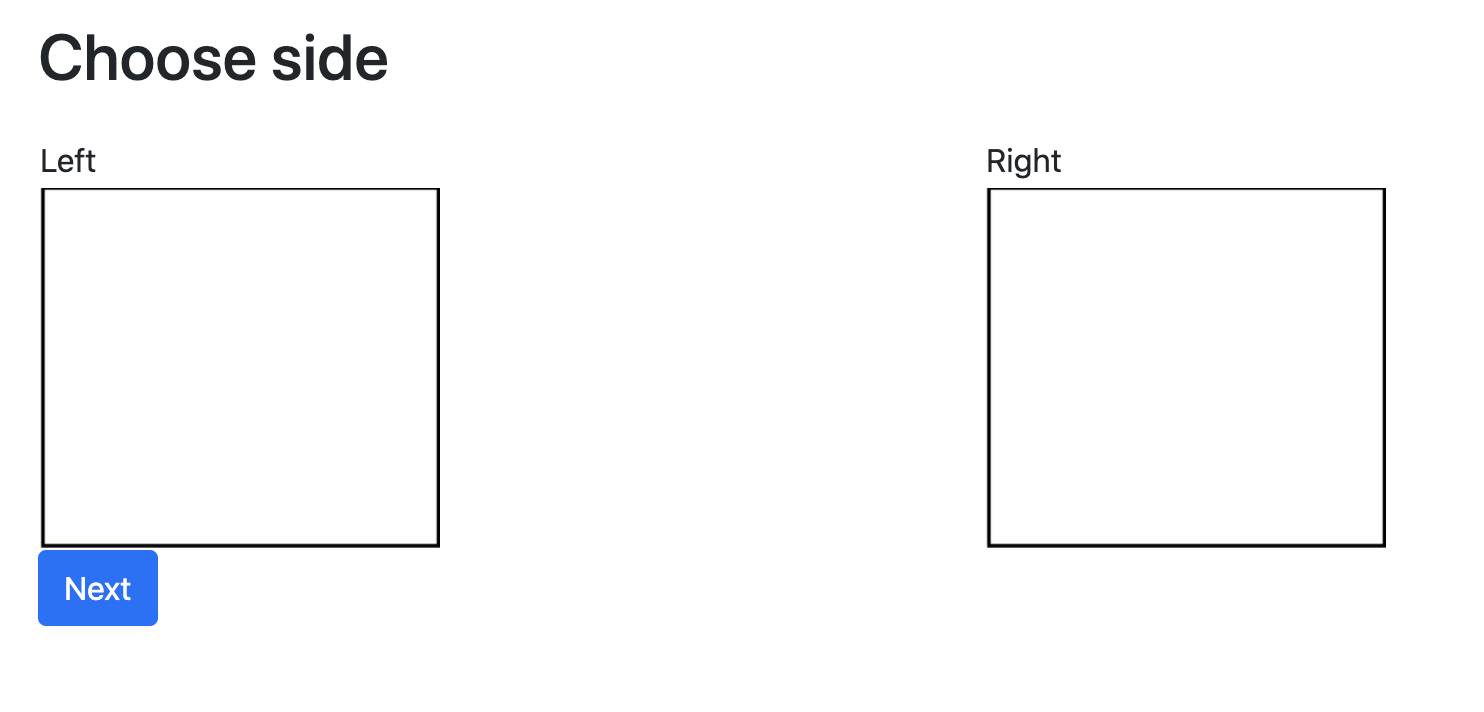
\includegraphics[scale=0.42]{first_stage.png}
	\end{figure}
	
	\begin{figure}[!h]
		\caption{Third stage in the "mind game"}
		\label{thirdstage}
		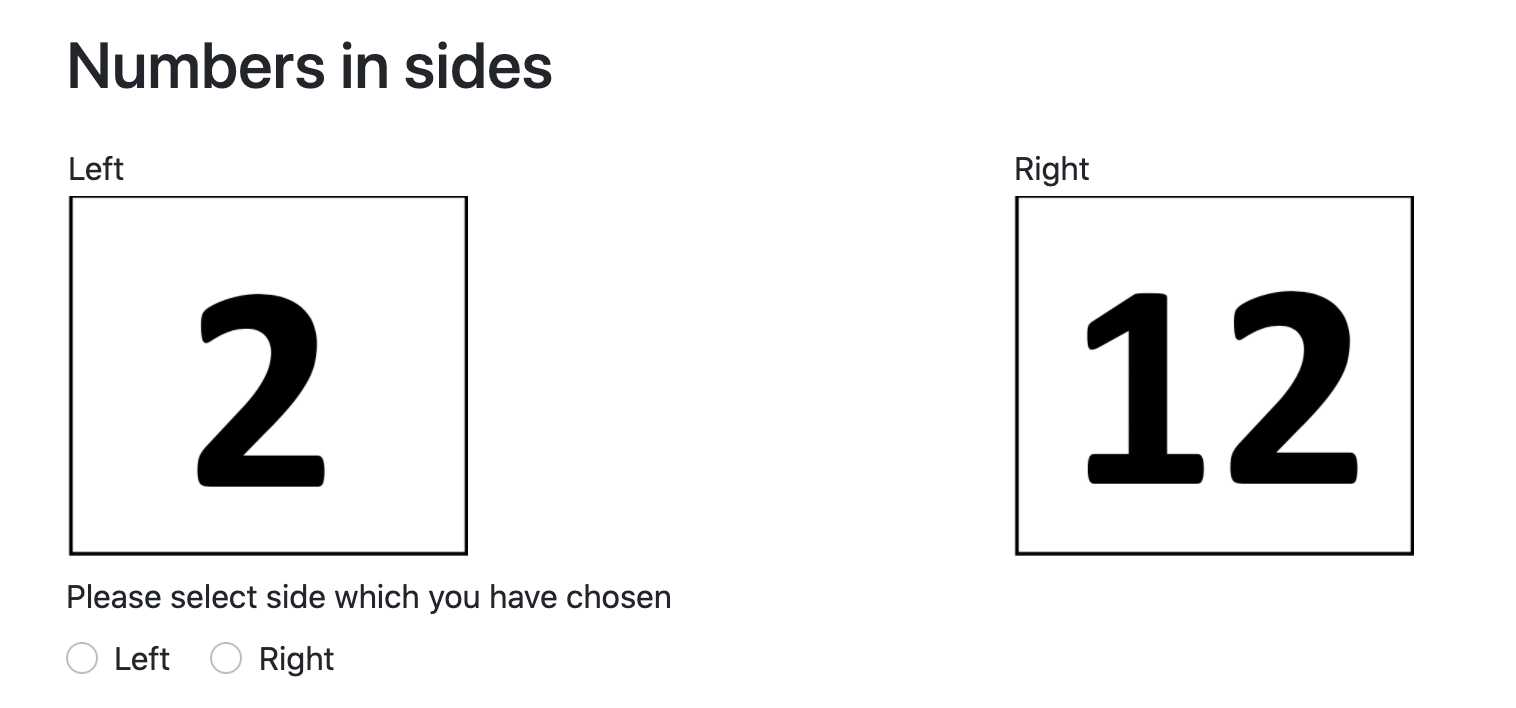
\includegraphics[scale=0.42]{third_stage.png}
	\end{figure}
	
	To measure deception level, \cite{jiang2013cheating} introduced \textit{foresight} binary variable which is equal 1 when participant choose the highest number and 0 otherwise. The variable \textit{Foresight} is equal to average of foresight over all rounds. If participant is honest and pick the side randomly, the \textit{Foresight} should be equal to 0.5, whereas if participant is cheater and always choose the highest number, the \textit{Foresight} should be equal to 1. Statistically identifiable cheaters defined as those who achieve improbably high individual foresight which examined by one-tailed test for Binomial distribution (in my experiment it is 7/8). \cite{jiang2013cheating, mol2020not} identified as cheaters more than 33\% participants (foresight level more than 0.67). Consequently, "mind game" introduces high incentives to cheat, and I assume to find many cheaters in my experiment for all treatments. To solve the problem of changing participants in groups for each round, I estimate for all 3 groups deception level as average \textit{foresight} in general and for each round (called \textit{Group Foresight per round} and \textit{Group Foresight}). Upward deviation from 0.5 for these variables demonstrates the dishonest performance in treatments. Based on the results of previous papers with "mind game" I assume two hypotheses.
	
	\vspace{0.2cm}
	
	\textbf{Hypothesis 6a:}
	\textit{More than 30\% participants will have \textit{Foresight} more than 7/8.}
	
	\textbf{Hypothesis 6b:}
	\textit{Group Foresight will be more than 67\% in all groups}
	
	\vspace{0.2cm}
	
	One more effect to analyze is the difference in numbers (a and b), because they can influence to intrinsic lying costs. \cite{kajackaite2015lying} found more cheating with higher payoffs. When participants saw that the benefit from deception is higher than possible lying costs, they switch to unethical behavior. Therefore, in treatments with 12 as highest number (when randomly chosen (a, b) is equal to (6,12) or (2,12) ) there will be more cheating, than the highest number is 6 (when randomly chosen (a, b) is equal to (6,12 ) ). Furthermore, lying costs are influenced by the outcome difference (the distance between what the agent observes and what he says) \autocite{gneezy2018lying}. Consequently, higher difference between randomly chosen a and b leads to higher dishonesty. To measure deception level for these treatments based on the pair of numbers (a and b) in rounds, I estimate average \textit{foresight} in general and for each round (called \textit{Treatment Foresight per round} and \textit{Treatment Foresight}). Upward deviation from 0.5 for these variables demonstrates the dishonest performance in treatments. 
	
	\vspace{0.2cm}
	
	\textbf{Hypothesis 7a:}
	\textit{Treatment Foresight in groups with numbers (2,12) and (6,12) will be higher than in treatment with numbers (2, 6)}
	
	\textbf{Hypothesis 7b:}
	\textit{Treatment Foresight in group with numbers (2,12) will be higher than in treatment with numbers (6, 12)}

	\vspace{0.2cm}
	
	The decision to use the same numbers in the lottery and "mind game" in each round concerned by simultaneous effects on lying costs and their possible substitution. In the lottery there was the influence on lying costs by changing perception of risk due to the result of the game with taking risk. In the "mind game" there was the influence on lying costs by the differences in payoffs. Therefore, if the numbers in both stage are not similar, the analyzing effects will be difficult to estimate or one of them will substitute other. For instance, if players lost 100, they have fewer incentives to cheat if they lost 1. Hence, in experiment numbers are the same in each round to analyze both effects simultaneously.
	
	
	\section{Results}\label{results}
		
	Table \ref{description} presents some descriptive experimental and questionnaire data: age, sex, gpa, income, cheat activity, cheat disagreement, subject risk, holt risk, average category person, \textit{Foresight}. There were 86 participants, most of them young people with high GPA (near 7.7 in average), high level of cheating disagreement (6.7 in average) and risk neutral (self-reported risk preferences near 6.1 in average). However, the Holt-Laury procedure demonstrated more risk aversion verified by low average category person (near 1.6, which means that people usually choose safe option in the lottery). \textit{Foresight} is more than 0.6 in average, in sample there is a person, who always select the highest and the lowest numbers. Therefore, in the "mind game" some participants cheated and the factors of dishonest behavior could be analyzed.
	
	\begin{table}[!htbp] \centering 
		  \caption{Descriptive statistics} 
		  \label{description} 
		\begin{tabular}{@{\extracolsep{-1pt}}lccccccc} 
		\hline \\[-1.8ex] 
		Statistic & \multicolumn{1}{c}{N} & \multicolumn{1}{c}{Mean} & \multicolumn{1}{c}{St. Dev.} & \multicolumn{1}{c}{Min} & \multicolumn{1}{c}{Pctl(25)} & \multicolumn{1}{c}{Pctl(75)} & \multicolumn{1}{c}{Max} \\ 
		\hline \\[-1.8ex] 
		age & 86 & 20.581 & 1.057 & 18 & 20 & 21 & 24 \\ 
		sex & 86 & 0.430 & 0.498 & 0 & 0 & 1 & 1 \\ 
		gpa & 86 & 7.698 & 1.128 & 5 & 7 & 8 & 10 \\ 
		income & 86 & 3.756 & 1.479 & 1 & 3 & 5 & 6 \\ 
		cheat activity & 86 & 3.837 & 2.201 & 1 & 2 & 5 & 10 \\ 
		cheat disagreement & 86 & 6.767 & 2.340 & 1 & 5 & 8 & 10 \\ 
		subject risk & 86 & 6.128 & 2.130 & 1 & 5 & 8 & 10 \\ 
		holt risk & 86 & 5.384 & 2.148 & 1 & 4 & 7 & 9 \\ 
		average category person& 86 & 1.664 & 0.590 & 1.000 & 1.000 & 2.125 & 3.000 \\ 
		\textit{Foresight} & 86 & 0.622 & 0.178 & 0.000 & 0.500 & 0.750 & 1.000 \\ 
		\hline \\[-1.8ex] 
		\end{tabular} 
	\end{table}


	Figure \ref{corr} shows Pearson's correlation coefficients for variables age, sex, gpa, income, cheat activity, cheat disagreement, subject risk, holt risk, average category person, \textit{Foresight}. There are three important messages. Cheat activity and cheat disagreement are negative correlated, which was expected, because if a person disagree with cheat activity he will cheat less. The measurements of risk seeking are highly correlated: self-reported perception of risk, estimation of risk seeking in the Holt-Laury procedure and average category person, which partially demonstrates the risk preferences in the lottery. Self-reported risk seeking is also correlated with \textit{Foresight}, which shows that risk seekers are prone to cheat more.
	
	
	\begin{figure}[!h]
	\caption{Pearson correlation coefficients}
	\label{corr}
	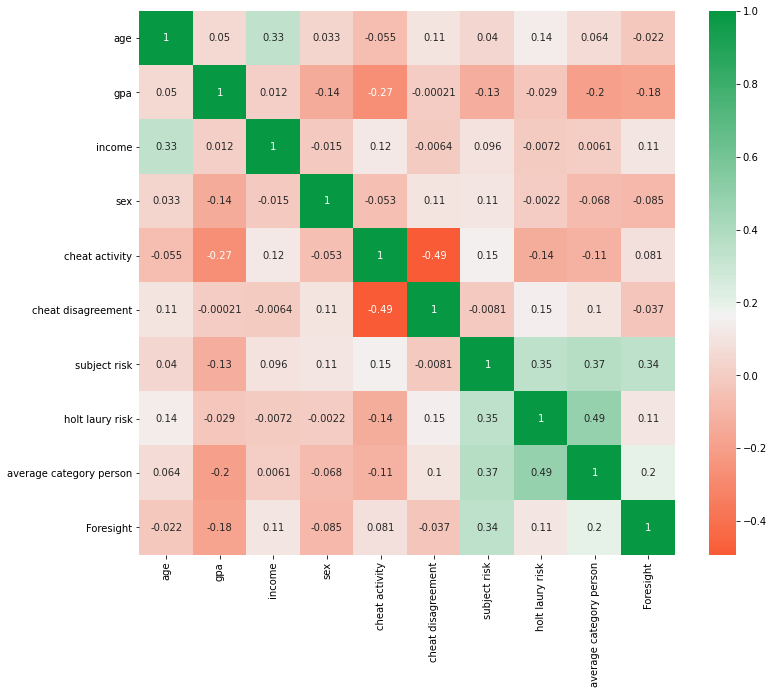
\includegraphics[scale=0.5]{corr.png}
	\end{figure}

	\begin{figure}[!h]
	\caption{Distribution of total foresight in experiment in relation to honest players}
	\label{hist}
	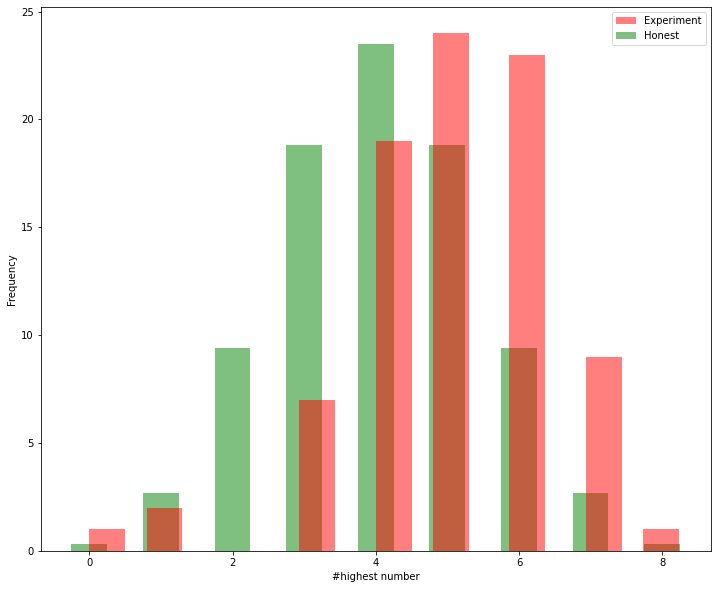
\includegraphics[scale=0.5]{hist1.png}
	\end{figure}

	To examine whether subjects cheated, I compare participants’ observed levels of foresight to the distribution of foresight levels I would expect if participants were honest. A normal approximation of the Binomial distribution is displayed in Figure \ref{hist}. The data indicates that 11.6\% (10/86) of the participants have a foresight level of 0.875 or higher: in at least 7 of the 8 rounds they click on the side with the highest number. If a participant is honest, the probability that he achieves this level is less than 5\% (one-tailed Binom test). However, the data indicates 38.3\% (33/86) of the participants have a foresight level of 0.75 or higher: in at least 6 of the 8 rounds they choose the highest number (the probability that he achieves this level is equal to 15\%). Consequently, I can conclude that 11\% of participants are identifiable cheaters and 27\% of participants are almost certainly offenders. This conclusion did not fully confirm Hypothesis 6a, which could be caused by few rounds. Nevertheless, the experiment presents the fact of cheating by some participants and I can analyze the reasons of unethical behavior.

	\begin{table}[!htbp] \centering 
		  \caption{Results of OLS regressions} 
		  \label{ols} 
		  \scriptsize
		\begin{tabular}{@{\extracolsep{5pt}}lccccccccc} 
		\\[-5ex]\hline 
		\hline \\[-1.8ex] 
		 & \multicolumn{8}{c}{\textit{Dependent variable:}} \\ 
		\cline{2-9} 
		\\[-1.8ex] & \multicolumn{4}{c}{\textit{Foresight}} & & \multicolumn{4}{c}{cheat activity} \\ 
		\\[-1.8ex] & (1) & (2) & (3) & (4) & | & (5) & (6) & (7) & (8)\\ 
		\hline \\[-1.8ex] 
		 age & $-$0.012 & $-$0.012 & $-$0.009 & $-$0.010 & |& $-$0.139 & $-$0.137 & $-$0.188 & $-$0.144 \\ 
		  & (0.019) & (0.019) & (0.018) & (0.018) & |& (0.235) & (0.234) & (0.233) & (0.228) \\ 
		 sex & $-$0.039 & $-$0.034 & $-$0.051 & $-$0.048& | & $-$0.395 & $-$0.457 & $-$0.438 & $-$0.597 \\ 
		  & (0.039) & (0.039) & (0.037) & (0.038) & |& (0.469) & (0.471) & (0.472) & (0.466) \\ 
		 gpa & $-$0.030$^{*}$ & $-$0.026 & $-$0.025 & $-$0.024 & |& $-$0.549$^{***}$ & $-$0.605$^{***}$ & $-$0.513$^{**}$ & $-$0.600$^{***}$ \\ 
		  & (0.017) & (0.018) & (0.016) & (0.017)& | & (0.207) & (0.212) & (0.209) & (0.207) \\ 
		 income & 0.016 & 0.016 & 0.011 & 0.012 & |& 0.215 & 0.217 & 0.211 & 0.189 \\ 
		  & (0.014) & (0.014) & (0.013) & (0.013) & |& (0.166) & (0.165) & (0.167) & (0.163) \\ 
		 average category person &  & 0.042 &  & 0.015 & |&  & $-$0.544 &  & $-$0.965$^{**}$ \\ 
		  &  & (0.038) &  & (0.034) & |&  & (0.459) &  & (0.423) \\ 
		 holt risk & 0.010 & 0.004 &  &  & |& $-$0.140 & $-$0.068 &  &  \\ 
		  & (0.009) & (0.010) &  &  & |& (0.109) & (0.124) &  &  \\ 
		 subject risk &  &  & 0.027$^{***}$ & 0.026$^{***}$ & |&  &  & 0.122 & 0.221$^{*}$ \\ 
		  &  &  & (0.009) & (0.009) & |&  &  & (0.111) & (0.116) \\ 
		 Constant & 0.999$^{**}$ & 0.927$^{**}$ & 0.812$^{**}$ & 0.799$^{**}$ & |& 11.048$^{**}$ & 11.967$^{**}$ & 10.299$^{**}$ & 11.218$^{**}$ \\ 
		  & (0.398) & (0.403) & (0.383) & (0.386) & |& (4.801) & (4.852) & (4.870) & (4.764) \\ 
		\hline \\[-1.8ex] 
		Observations & 86 & 86 & 86 & 86 & |& 86 & 86 & 86 & 86 \\ 
		R$^{2}$ & 0.073 & 0.087 & 0.163 & 0.165 & |& 0.120 & 0.135 & 0.115 & 0.170 \\ 
		\hline 
		\hline \\[-1.8ex] 
		\textit{Note:}  & \multicolumn{8}{r}{$^{*}$p$<$0.1; $^{**}$p$<$0.05; $^{***}$p$<$0.01} \\ 
		\end{tabular} 
	\end{table}

	To test hypotheses, I used Ordinary Least Squares (OLS) regressions with data from questionnaires and \textit{Foresight}. The results of regressions are presented in the Table \ref{ols}. I found that self-reported risk seeking is significant and positive for \textit{Foresight} (Hypothesis 1 is approved). It indicates that risk seekers cheat more. However, the significance of it is less when dependent variable is self-reported cheat activity (it is significant with  p-value 10\%). Moreover, in that regressions GPA becomes negatively significant, while it was not in regressions with self-reported risk seeking as dependent variable. Therefore, Hypothesis 2 is rejected, which could be caused by less level of \textit{Foresight} (I called this reason as "honest sample") and self-selected cheat activity. Another consequence of "honest sample" in the experiment is that there is no significance of variables  \textit{age, sex, income} in all regressions (Hypotheses 3a, 3b, 3d are not approved). Although the level of cumulative GPA has negative influence in regressions with self-reported cheat activity as dependent variable (Hypothesis 3c is partially approved). The last result of these regressions is the measurement of risk-seeking in the Holt-Laury procedure is not significant (Hypothesis 4 is not approved). It could be caused by separate scale of payoffs in the Holt-Laury task and "mind game" (1,16,20,38 in the first and 2,6,12 in the second), so participants' perception of risk in "mind game" differs from reported in the Holt-Laury procedure. 
	
	To test hypotheses in individual level, I use panel regressions with Random Effect where dependent variable was binary \textit{foresight}. Results are presented in Table \ref{panelreg}. In panel regressions the results from OLS regressions with average \textit{foresight} are repeated. Self-reported risk seeking has significantly positive effect to \textit{foresight} and Hypothesis 1 is approved. However, Hypotheses 3a, b, c, d are not approved which could be caused by small variation in sample and "honest sample". Otherwise, I found that the group number has positive and significant influence on \textit{foresight} with p-value 10\%. Hence, incentivized person will cheat more and Hypotheses 5a,b  are partially approved, because it will be caused by few participants in group who chose risk option and won (incentivized).

	\begin{table}[!htbp] \centering 
		  \caption{Results of panel regressions with Random Effect (RE)} 
		  \label{panelreg} 
		  \scriptsize
		\begin{tabular}{@{\extracolsep{5pt}}lccccccc} 
		\\[-1.8ex]\hline 
		\hline \\[-1.8ex] 
		 & \multicolumn{7}{c}{\textit{Dependent variable:}} \\ 
		\cline{2-8} 
		\\[-1.8ex] & \multicolumn{7}{c}{\textit{foresight}} \\ 
		\\[-1.8ex] & (1) & (2) & (3) & (4) & (5) & (6) & (7)\\ 
		\hline \\[-1.8ex] 
		 age & $-$0.011 & $-$0.010 & $-$0.009 & $-$0.012 & $-$0.012 & $-$0.012 & $-$0.011 \\ 
		  & (0.019) & (0.019) & (0.019) & (0.020) & (0.019) & (0.020) & (0.019) \\ 
		 sex & 0.046 & 0.046 & 0.051 & 0.034 & 0.034 & 0.039 & 0.034 \\ 
		  & (0.038) & (0.038) & (0.038) & (0.039) & (0.039) & (0.039) & (0.039) \\ 
		 gpa & $-$0.023 & $-$0.022 & $-$0.025 & $-$0.026 & $-$0.026 & $-$0.030$^{*}$ & $-$0.026 \\ 
		  & (0.017) & (0.017) & (0.017) & (0.017) & (0.017) & (0.017) & (0.017) \\ 
		 income & 0.012 & 0.012 & 0.012 & 0.016 & 0.016 & 0.016 & 0.016 \\ 
		  & (0.013) & (0.013) & (0.013) & (0.014) & (0.014) & (0.014) & (0.014) \\ 
		 treatment number & 0.020 &  & 0.019 & 0.022 &  & 0.020 & 0.022 \\ 
		  & (0.022) &  & (0.022) & (0.023) &  & (0.023) & (0.023) \\ 
		 group number& 0.028 & 0.027 &  & 0.040$^{*}$ & 0.039$^{*}$ &  & 0.043$^{*}$ \\ 
		  & (0.023) & (0.023) &  & (0.024) & (0.024) &  & (0.022) \\ 
		 subject risk & 0.024$^{***}$ & 0.025$^{***}$ & 0.027$^{***}$ &  &  &  &  \\ 
		  & (0.009) & (0.009) & (0.009) &  &  &  &  \\ 
		 holt risk &  &  &  & 0.004 & 0.004 & 0.009 &  \\ 
		  &  &  &  & (0.010) & (0.010) & (0.009) &  \\ 
		 Constant & 0.706$^{*}$ & 0.740$^{*}$ & 0.730$^{*}$ & 0.859$^{**}$ & 0.899$^{**}$ & 0.925$^{**}$ & 0.852$^{**}$ \\ 
		  & (0.392) & (0.390) & (0.391) & (0.403) & (0.399) & (0.402) & (0.401) \\ 
		\hline \\[-1.8ex] 
		Observations & 688 & 688 & 688 & 688 & 688 & 688 & 688 \\ 
		R$^{2}$ & 0.025 & 0.024 & 0.023 & 0.014 & 0.013 & 0.010 & 0.014 \\ 
		\hline 
		\hline \\[-1.8ex] 
		\textit{Note:}  & \multicolumn{7}{r}{$^{*}$p$<$0.1; $^{**}$p$<$0.05; $^{***}$p$<$0.01} \\ 
		\end{tabular} 
	\end{table} 

	
	\begin{figure}[!htb]
		\caption{Trends of Foresight over 8 rounds, by group (high) and by treatment (low)}\label{dynamics}
		\begin{minipage}{0.6\textwidth}
			\centering
			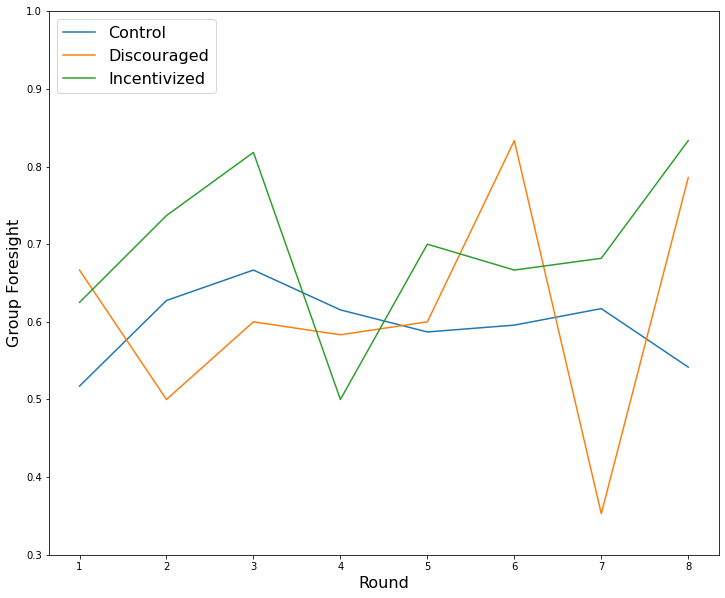
\includegraphics[width=.99\linewidth]{rounds_person.png}
		\end{minipage}
	\begin{minipage}{0.6\textwidth}
		\centering
		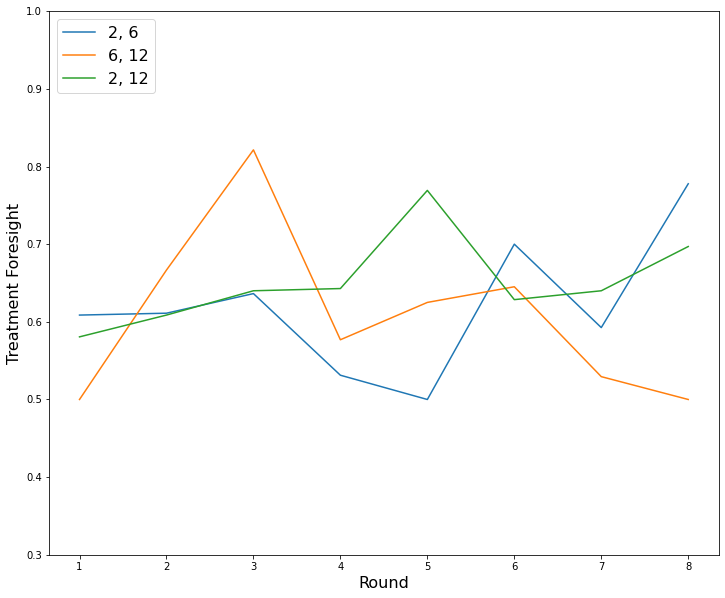
\includegraphics[width=.99\linewidth]{rounds_num.png}
	\end{minipage}
	\end{figure}
 	 
 	 To more accurate test Hypotheses 5-7 I estimate average \textit{Group Foresight} and \textit{Treatment Foresight} over rounds. Figure \ref{dynamics} shows the trends of them over 8 rounds.
 	
 	The \textit{Group Foresight} in incentivized group is equal to 0.7 in average and is the highest in almost all rounds (Hypothesis 5a is approved), whereas the \textit{Group Foresight} in discouraged and control groups are equal to 0.6 in average and varied. Hence, Hypothesis 6b is not approved, which will be caused by few round and "honest sample". Furthermore, \textit{Group Foresight} in discouraged is not the lowest in many rounds (Hypothesis 5b is not approved), because participants did not lose anything actually, the differences between possible outcomes were not significant and in discouraged and incentivized group there were few participants. However, in the 6 round in discouraged group \textit{Foresight} is the least and lower than 0.4, which demonstrates that in this round the affect to perception of risk could be the highest and participants did not have incentives to cheat (most of the participants in this round have the pair (2,12), when the effect of difference in outcomes is the highest). 
 	
 	
 	Considering the trends of \textit{Foresight} by treatment, observed variance is lower and results are debatable. In the first 3 rounds the \textit{Foresight} in treatment with (6, 12) was the highest, while after the 4 round it decreased dramatically from 0.8 in the third round to 0.5 in the last round (this trend partially approves Hypothesis 7a). Moral balancing can explain this downtrend, according to which ‘bad’ behavior in the past is compensated by ‘good’ behavior now \autocite{mazar2010green}, so participants cheated more in the first rounds and in the last rounds tried to find moral balance and behave honestly. However, in other treatments it is seen \textit{Foresight} more than 0.6 and fluctuated growing over rounds, so in these treatments participants also tried to find moral balance, but for them ‘good’ behavior in the past is compensated by ‘bad’ behavior now \autocite{clot2014smug}. Basically, \textit{Foresight} in treatments (2, 12) and (2, 6) are partially identical in the first 3 and last 3 rounds, but in the 4 and 5 rounds \textit{Foresight} in treatment (2, 12) is higher than in treatment (2, 6). This trend partially confirms Hypothesis 7b, because due to moral balancing of participants and convergence in the first and last rounds it is not approved absolutely.
 	
 	The trends of Foresight over 8 rounds, by group and treatment shows high variance and possible joint affects by group and treatment, hence it is necessary to split them and analyze \textit{Foresight} simultaneously. Figure \ref{main_hist} demonstrates \textit{Foresight} by group and treatment.
 	
	\begin{figure}[!h]
		\caption{Foresight by group and treatment }
		\label{main_hist}
		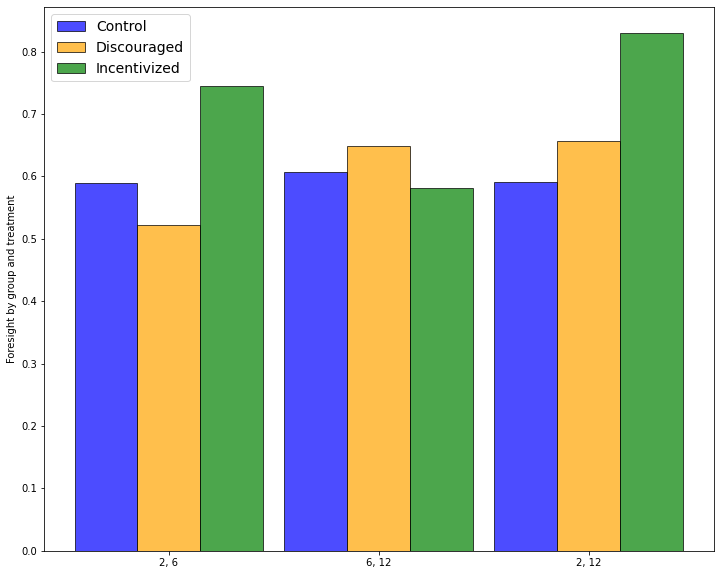
\includegraphics[scale=0.58]{num_person.png}
	\end{figure}
	
	In the treatment with (2, 12) there is the highest \textit{Foresight} in discouraged and incentivized groups. In this treatment the effects of groups are clearly observed: in the incentivized group is the highest \textit{Foresight}, whereas in the control group is the lowest and partially equal to \textit{Foresight} in the discouraged group. In the treatment (2, 6) \textit{Foresight} in the incentivized group is also the highest and in the discouraged group is the lowest. Though in the treatment (2, 6) \textit{Foresight} in groups are almost equal. Consequently, the influence on the perception of risk by the choice and result in the lottery is fully observed when the smaller number is the lowest. Therefore, the payoff of honest behavior (in experiment it is lower number) increases the effect to lying costs by changing in perception of risk. 

	In the incentivized group \textit{Foresight} is the highest in the treatment with (2, 12) and (2, 6), while it is lower than \textit{Foresight} in the discouraged group for treatment with (6, 12). In the control group \textit{Foresight} is almost equal for all treatments (almost 0.6). In the discouraged group \textit{Foresight} grows with the difference between payoffs, so the effect to perception of risk is decreasing with more outcome difference. Hence, the influence on lying costs by increasing risk aversion is reducing with more differences between outcomes, and it is maximum when the payoff difference is the lowest.

	
	\printbibliography

	
\end{document}